\documentclass[a3paper,xelatex,english]{bxjsarticle}
\usepackage{pgfplots,pgfplotstable}
\pgfplotsset{ compat = newest }
\usepackage{tikz}
\usetikzlibrary{arrows.meta,bending,calc,shapes,positioning}
\usepackage{ascmac}
\usepackage{fancybox}
\usepackage{amsmath,amssymb}
\usepackage{algorithm}
\usepackage[edges]{forest}
\usepackage{array}
\usepackage{algpseudocode}
\usepackage{paralist}
\usepackage{cases}
\usepackage{fvextra}
\usepackage{colortbl}
\usepackage{xcolor}
\usepackage{fancyhdr}
\usepackage[explicit]{titlesec}
\usepackage{xspace}
\usepackage[many]{tcolorbox}
\usepackage{lastpage}
\usepackage{verbatim}
\usepackage{multirow}
\usepackage{censor}
\usepackage[unicode,pdftitle={Report of Entropy estimates based on NIST SP 800-90B non-IID track},setpagesize=false]{hyperref}
\usepackage[open,openlevel=4]{bookmark}
\newcommand\mib[1]{\boldsymbol{#1}}
\usepgfplotslibrary{patchplots}
%%%%%%%%%%%%%%%%%%%%%%%%%%%%%%%%%%%%%%%%%%%%%%%%%%%%%%%%%%%%%%%%%%%%%%%%%%%%%%%
%%%%%%
%%%%%% customize page numbering
%%%%%%
%%%%%%%%%%%%%%%%%%%%%%%%%%%%%%%%%%%%%%%%%%%%%%%%%%%%%%%%%%%%%%%%%%%%%%%%%%%%%%%
\fancypagestyle{mypagestylewithtotalpagenumbers}{
\lhead{}
\rhead{}
\cfoot{\thepage/\pageref{LastPage}}
\renewcommand{\headrulewidth}{0.0pt}
}
%%%%%%%%%%%%%%%%%%%%%%%%%%%%%%%%%%%%%%%%%%%%%%%%%%%%%%%%%%%%%%%%%%%%%%%%%%%%%%%
%%%%%%
%%%%%% output up to 4-th level
%%%%%%
%%%%%%%%%%%%%%%%%%%%%%%%%%%%%%%%%%%%%%%%%%%%%%%%%%%%%%%%%%%%%%%%%%%%%%%%%%%%%%%
\setcounter{secnumdepth}{4}
\setcounter{tocdepth}{4}
\setlength{\topmargin}{-1cm}
\setlength{\textheight}{37cm}
%%%%%%%%%%%%%%%%%%%%%%%%%%%%%%%%%%%%%%%%%%%%%%%%%%%%%%%%%%%%%%%%%%%%%%%%%%%%%%%
%%%%%%
%%%%%%
%%%%%%
%%%%%%%%%%%%%%%%%%%%%%%%%%%%%%%%%%%%%%%%%%%%%%%%%%%%%%%%%%%%%%%%%%%%%%%%%%%%%%%
%%%\renewcommand{ \figurename }{Figure }
%%%\renewcommand{ \tablename }{Table }
%%%\renewcommand{ \refname }{References}
%%%%%%%%%%%%%%%%%%%%%%%%%%%%%%%%%%%%%%%%%%%%%%%%%%%%%%%%%%%%%%%%%%%%%%%%%%%%%%%
%%%%%%
%%%%%%
%%%%%%
%%%%%%%%%%%%%%%%%%%%%%%%%%%%%%%%%%%%%%%%%%%%%%%%%%%%%%%%%%%%%%%%%%%%%%%%%%%%%%%
\definecolor{rowcolorlightblue}{RGB}{191,233,251}
\definecolor{bordercolordarkblue}{RGB}{0,163,243}
\definecolor{BleuDur}{RGB}{27,61,176}
\definecolor{Nigelle}{RGB}{0,133,201}
\definecolor{BleuFaience}{RGB}{105,171,219}
\definecolor{anotherlightblue}{RGB}{61,143,244}
%%%%%%%%%%%%%%%%%%%%%%%%%%%%%%%%%%%%%%%%%%%%%%%%%%%%%%%%%%%%%%%%%%%%%%%%%%%%%%%
%%%%%%
%%%%%%
%%%%%%
%%%%%%%%%%%%%%%%%%%%%%%%%%%%%%%%%%%%%%%%%%%%%%%%%%%%%%%%%%%%%%%%%%%%%%%%%%%%%%%
\def\chpcolor{BleuDur}
\def\chpcolortxt{BleuDur}
\def\sectionfont{\sffamily\LARGE}
%%%%%%%%%%%%%%%%%%%%%%%%%%%%%%%%%%%%%%%%%%%%%%%%%%%%%%%%%%%%%%%%%%%%%%%%%%%%%%%
%%%%%%
%%%%%%
%%%%%%
%%%%%%%%%%%%%%%%%%%%%%%%%%%%%%%%%%%%%%%%%%%%%%%%%%%%%%%%%%%%%%%%%%%%%%%%%%%%%%%
\makeatletter
%Section:
\def\@sectionstrut{\vrule\@width\z@\@height12.5\p@}
\def\@makesectionhead#1{%
  {\par\vspace{20pt}%
   \parindent 0pt\raggedleft\sectionfont
   \colorbox{\chpcolor}{%
     \parbox[t]{90pt}{\color{white}\@sectionstrut\@depth4.5\p@\hfill
       \ifnum\c@secnumdepth>\z@\thesection\fi}%
   }%
   \begin{minipage}[t]{\dimexpr\textwidth-90pt-2\fboxsep\relax}
   \color{\chpcolortxt}\@sectionstrut\hspace{5pt}#1
   \end{minipage}\par
   \vspace{10pt}%
  }
}
\def\section{\@afterindentfalse\secdef\@section\@ssection}
\def\@section[#1]#2{%
  \ifnum\c@secnumdepth>\m@ne
    \refstepcounter{section}%
    \addcontentsline{toc}{section}{\protect\numberline{\thesection}#1}%
  \else
    \phantomsection
    \addcontentsline{toc}{section}{#1}%
  \fi
  \sectionmark{#1}%
  \if@twocolumn
    \@topnewpage[\@makesectionhead{#2}]%
  \else
    \@makesectionhead{#2}\@afterheading
  \fi
}
\def\@ssection#1{%
  \if@twocolumn
    \@topnewpage[\@makesectionhead{#1}]%
  \else
    \@makesectionhead{#1}\@afterheading
  \fi
}
\makeatother
%%%%%%%%%%%%%%%%%%%%%%%%%%%%%%%%%%%%%%%%%%%%%%%%%%%%%%%%%%%%%%%%%%%%%%%%%%%%%%%
%%%%%%
%%%%%%
%%%%%%
%%%%%%%%%%%%%%%%%%%%%%%%%%%%%%%%%%%%%%%%%%%%%%%%%%%%%%%%%%%%%%%%%%%%%%%%%%%%%%%
\setlength{ \topmargin }{-1.5cm}
%%%%%%%%%%%%%%%%%%%%%%%%%%%%%%%%%%%%%%%%%%%%%%%%%%%%%%%%%%%%%%%%%%%%%%%%%%%%%%%
%%%%%%
%%%%%%
%%%%%%
%%%%%%%%%%%%%%%%%%%%%%%%%%%%%%%%%%%%%%%%%%%%%%%%%%%%%%%%%%%%%%%%%%%%%%%%%%%%%%%
\pagestyle{mypagestylewithtotalpagenumbers}
%%%%%%
%%%%%%
%%%%%%
\title{Report of Entropy estimates based on NIST SP 800-90B non-IID track}
\date{2023-Nov-24 21:18:48.140359}
\begin{document}
\StopCensoring
\maketitle
%%%%%%%%%%%%%%%%%%%%%%%%%%%%%%%%%%%%%%%%%%%%%%%%%%%%%%%%%%%%%%%%%%%%%%%%%%%%%%%
%%%%%%
%%%%%%%%%%%%%%%%%%%%%%%%%%%%%%%%%%%%%%%%%%%%%%%%%%%%%%%%%%%%%%%%%%%%%%%%%%%%%%%
\thispagestyle{mypagestylewithtotalpagenumbers}
%%%%%%%%%%%%%%%%%%%%%%%%%%%%%%%%%%%%%%%%%%%%%%%%%%%%%%%%%%%%%%%%%%%%%%%%%%%%%%%
%%%%%%
%%%%%%%%%%%%%%%%%%%%%%%%%%%%%%%%%%%%%%%%%%%%%%%%%%%%%%%%%%%%%%%%%%%%%%%%%%%%%%%
\section{Identification information}
\subsection{Identification of acquisition data from entropy source}
\renewcommand{\arraystretch}{1.8}
\begin{table}[h]
\caption{Identification information of acquisition data from entropy source}
\begin{center}
\begin{tabular}{|>{\columncolor{anotherlightblue}}p{2cm}|p{20.5cm}|}
\hline 
Path to the acquisition data & \verb|"C:\usr\01_git_repos\NIST_SP800-90B_EntropyAssessment\SP800-90B_EntropyAssessment\bin\rand8_short.bin"| \\
\hline
SHA-256 hash value of the acquisition data [hex] & 
\begin{verbatim}
17d2eaf9 544cd6ae a3e245be c362f494 376d0b1c a6140c47 5a35f1ad 1f8c2803
\end{verbatim} 
\\
\hline
Last write time & 2023-Jun-30 21:13:46 \\
\hline
\end{tabular}
\end{center}
\end{table}
\renewcommand{\arraystretch}{1.8}
\begin{itemize}
		\item Name of the submitter of the acquisition data : 
		    \begin{Form}
		    \noindent
		    \TextField[name=NameOfSubmitter, multiline=false, bordercolor=bordercolordarkblue,width=12cm]{}
		    \end{Form}
		\item Brief explanation of the acquisition data (or entropy source) : \\
		    \begin{Form}
		    \noindent
		    \TextField[name=ExplanationOfAcquisitionData, multiline=true, bordercolor=bordercolordarkblue,width=\linewidth,height=1in]{}
		    \end{Form}
	\end{itemize} 
\subsection{Identification of analysis environment}
\renewcommand{\arraystretch}{1.8}
\begin{table}[h]
\caption{Identification information of analysis environment}
\begin{center}
\begin{tabular}{|>{\columncolor{anotherlightblue}}l|>{\columncolor{anotherlightblue}}l|p{12cm}|}
\hline 
Analysis tool & Name & Another entropy estimation tool with extensions \\
\cline{2-3}
\, & Versioning information & 1.0.50 \\
\cline{2-3}
\, & built as &  64-bit application \\
\cline{2-3}
\, & built by &  Intel C++ Compiler ( \verb|__INTEL_LLVM_COMPILER|: 20240000 ) \\
\cline{2-3}
\, & linked libraries &  Boost C++ 1.83.0 \\
\hline
Analysis environment & Hostname & \censor{TIGER140A} \\
\cline{2-3}
\, & CPU information & AMD Ryzen 5 PRO 5650U with Radeon Graphics      \\
\cline{2-3}
\, &  Physical memory size & 47950 MiB \\
\cline{2-3}
\, &  OS information & Windows 10 or greater 64-bit \\
\cline{2-3}
\, &  Username & \censor{genya} \\
\hline
\end{tabular}
\end{center}
\end{table}
\renewcommand{\arraystretch}{1.4}
\subsection{Identification of analysis conditions}
\renewcommand{\arraystretch}{1.8}
\begin{table}[h]
\caption{Identification information of analysis conditions}
\begin{center}
\begin{tabular}{|>{\columncolor{anotherlightblue}}l|p{8cm}|}
\hline 
Number of samples & 10000 \\
\hline
Bits per sample & 8 \\
\hline
Byte to bit conversion & 
Most Significant bit (MSb) first
 \\
\hline
\end{tabular}
\end{center}
\end{table}
\renewcommand{\arraystretch}{1.4}
\subsection{Identification of analysis method}
NIST SP 800-90B \cite{SP80090B} 6.3 with corrections \cite{CorrectionsSP80090B} is applied
\clearpage
\section{Executive summary}
\subsection{Numerical results of min-entropy estimates based on non-IID track}
\pgfplotstableread{
section	y	y-min	y-max
6.3.1	 7.01045	0.0218983	       0
6.3.5	 7.01045	       0	       0
6.3.6	  7.2892	       0	       0
6.3.7	 7.37519	0.0284959	0.0291266
6.3.8	 6.63644	  1.6672	 1.36356
6.3.9	 7.32763	0.0273146	0.0278925
6.3.10	 7.41098	0.0291267	0.0297867
}{\summarytableNonBinary}
\pgfplotstableread{
section	y	y-min	y-max
6.3.1	0.983387	3.56541e-05	       0
6.3.2	0.832053	0.000971685	0.00097834
6.3.3	0.997725	7.12807e-05	       0
6.3.4	0.732612	       0	       0
6.3.5	0.910786	       0	       0
6.3.6	 0.98193	       0	       0
6.3.7	0.994537	3.59607e-05	3.59616e-05
6.3.8	0.989693	3.58113e-05	3.58122e-05
6.3.9	0.987815	3.57647e-05	3.57656e-05
6.3.10	0.988082	3.57781e-05	3.5779e-05
}{\summarytableBinary}
\begin{table}[h]
\caption{Numerical results}
\begin{center}
\begin{tabular}{|l|c|c|c|c|}
\hline 
\rowcolor{anotherlightblue} %%
Estimator										& $H_{\textrm{original}}$$^{\textrm{\,a}}$			& Notes to $H_{\textrm{original}}$  & $H_{\textrm{bitstring}}$$^{\textrm{\,b}}$	& Notes to $H_{\textrm{bitstring}}$			\\ 
\cline{2-5}
\rowcolor{anotherlightblue} %%
\,												& [bit / 8 - bit] & \, & [bit / 1 - bit] &	\,	\\
\hline 
The Most Common Value Estimate					& 7.01045& see \ref{sec:NonBinary631} & 0.983387& see \ref{sec:Binary631} \\
\hline 
The Collision Estimate							& ---		  & --- & 0.832053& see \ref{sec:Binary632} \\
\hline 
The Markov Estimate								& ---		  & --- & 0.997725& see \ref{sec:Binary633} \\
\hline 
The Compression Estimate						& ---		  & --- & 0.732612& see \ref{sec:Binary634} \\
\hline 
The t-Tuple Estimate							& 7.01045& see \ref{sec:NonBinary635} & 0.910786& see \ref{sec:Binary635} \\
\hline 
The Longest Repeated Substring (LRS) Estimate	& 7.2892& see \ref{sec:NonBinary636} & 0.98193& see \ref{sec:Binary636} \\
\hline 
Multi Most Common in Window Prediction Estimate	& 7.37519& see \ref{sec:NonBinary637} & 0.994537& see \ref{sec:Binary637} \\
\hline 
The Lag Prediction Estimate						& 6.63644& see \ref{sec:NonBinary638} & 0.989693& see \ref{sec:Binary638} \\
\hline 
The MultiMMC Prediction Estimate				& 7.32763& see \ref{sec:NonBinary639} & 0.987815& see \ref{sec:Binary639} \\
\hline 
The LZ78Y Prediction Estimate					& 7.41098& see \ref{sec:NonBinary6310} &0.988082& see \ref{sec:Binary6310} \\
\hline \hline 
The intial entropy source estimate [bit / 8 - bit]	& \multicolumn{4}{|c|}{5.86089}	\\
$H_{I} = \min (H_{\textrm{original}}, 8\times H_{\textrm{bitstring}})$ &\multicolumn{4}{ | c | } {\, }	\\
\hline \hline 
\multicolumn{5}{|l|}{$^{\,a}$\quad Entropy estimate of the sequential dataset [source: NIST SP 800-90B \cite{SP80090B} 3.1.3]} \\
\multicolumn{5}{|l|}{$^{\,b}$\quad An additional entropy estimation (per bit) for the non-binary sequential dataset [see NIST SP 800-90B \cite{SP80090B} 3.1.3]} \\
\hline 
\end{tabular}
\end{center}
\end{table}
\clearpage
\subsection{Visual comparison of min-entropy estimates from original samples}
\begin{figure}[htbp]
\centering

\begin{tikzpicture} 
\begin{axis}
	[symbolic x coords={6.3.1,6.3.2,6.3.3,6.3.4,6.3.5,6.3.6,6.3.7,6.3.8,6.3.9,6.3.10},
	width=18cm,
	ymin=0,
	ymax=8,
	xlabel=Sub-sub-section of NIST SP 800-90B,
	ylabel={Estimated min-entropy $[$bit / 8-bit$]$},
	xtick=data]
\addplot+[forget plot,only marks] 
  plot[error bars/.cd, y dir=both, y explicit]
  table[x=section,y=y,y error plus expr=\thisrow{y-max},y error minus expr=\thisrow{y-min}] {\summarytableNonBinary};
\addplot+[Nigelle,no marks,sharp plot,update limits=false] 
coordinates {(6.3.1,6.63644) (6.3.10,6.63644)}
node[below] at (axis cs:6.3.5,6.63644) {Estimated min-entropy = 
6.63644};
\end{axis} 
\end{tikzpicture}

\caption{Estimated Min-Entropy using $\S$6.3 of NIST SP 800-90B}
\end{figure}
\subsection{Visual comparison of min-entropy estimates by interpreting each sample as bitstring}
\begin{figure}[htbp]
\centering

\begin{tikzpicture} 
\begin{axis}
	[symbolic x coords={6.3.1,6.3.2,6.3.3,6.3.4,6.3.5,6.3.6,6.3.7,6.3.8,6.3.9,6.3.10},
	width=18cm,
	ymin=0,
	ymax=1,
	xlabel=Sub-sub-section of NIST SP 800-90B,
	ylabel={Estimated min-entropy $[$bit / 1-bit$]$},
	xtick=data]
\addplot+[forget plot,only marks] 
  plot[error bars/.cd, y dir=both, y explicit]
  table[x=section,y=y,y error plus expr=\thisrow{y-max},y error minus expr=\thisrow{y-min}] {\summarytableBinary};
\addplot+[Nigelle,no marks,sharp plot,update limits=false] 
coordinates {(6.3.1,0.732612) (6.3.10,0.732612)}
node[below] at (axis cs:6.3.5,0.732612) {Estimated min-entropy = 
0.732612};
\end{axis} 
\end{tikzpicture}

\caption{Estimated Min-Entropy using $\S$6.3 of NIST SP 800-90B}
\end{figure}
\clearpage
\section{Detailed results of analysis from original samples}
\subsection{The Most Common Value Estimate (NIST SP 800-90B Section 6.3.1)}\label{sec:NonBinary631}

\begin{figure}[htbp]
\centering

\begin{tikzpicture}
\begin{axis}[
	ybar,
	bar width=1.25pt,
	xmin=-0.125,
xmax=255.125,	ymin=0,
	width=20cm,
	xlabel=$x_i$,
	ylabel=\#$\{x_i \,\textrm{in} \,S\} / L$
]
\addplot coordinates {
(       0,   0.0029)
(       1,   0.0042)
(       2,   0.0035)
(       3,   0.0042)
(       4,   0.0036)
(       5,   0.0047)
(       6,    0.004)
(       7,   0.0035)
(       8,   0.0044)
(       9,   0.0043)
(      10,   0.0036)
(      11,   0.0042)
(      12,   0.0041)
(      13,   0.0042)
(      14,   0.0032)
(      15,   0.0034)
(      16,   0.0036)
(      17,   0.0041)
(      18,   0.0042)
(      19,   0.0028)
(      20,   0.0043)
(      21,   0.0045)
(      22,   0.0024)
(      23,   0.0034)
(      24,    0.003)
(      25,   0.0035)
(      26,   0.0041)
(      27,   0.0033)
(      28,    0.004)
(      29,   0.0036)
(      30,   0.0044)
(      31,   0.0038)
(      32,   0.0044)
(      33,    0.005)
(      34,   0.0044)
(      35,   0.0038)
(      36,    0.005)
(      37,   0.0037)
(      38,   0.0042)
(      39,   0.0045)
(      40,   0.0046)
(      41,   0.0041)
(      42,   0.0035)
(      43,   0.0038)
(      44,   0.0033)
(      45,    0.004)
(      46,   0.0049)
(      47,   0.0035)
(      48,   0.0046)
(      49,   0.0039)
(      50,    0.004)
(      51,   0.0034)
(      52,   0.0039)
(      53,   0.0032)
(      54,   0.0047)
(      55,   0.0055)
(      56,   0.0034)
(      57,   0.0029)
(      58,   0.0038)
(      59,   0.0038)
(      60,   0.0042)
(      61,   0.0034)
(      62,    0.005)
(      63,   0.0036)
(      64,    0.004)
(      65,   0.0039)
(      66,   0.0033)
(      67,   0.0048)
(      68,   0.0032)
(      69,   0.0046)
(      70,   0.0042)
(      71,   0.0044)
(      72,   0.0037)
(      73,   0.0047)
(      74,   0.0042)
(      75,   0.0037)
(      76,   0.0049)
(      77,   0.0031)
(      78,   0.0036)
(      79,   0.0045)
(      80,   0.0037)
(      81,   0.0031)
(      82,   0.0038)
(      83,   0.0046)
(      84,   0.0035)
(      85,    0.004)
(      86,   0.0034)
(      87,   0.0046)
(      88,   0.0039)
(      89,   0.0052)
(      90,   0.0035)
(      91,   0.0042)
(      92,   0.0046)
(      93,   0.0039)
(      94,    0.005)
(      95,   0.0024)
(      96,    0.003)
(      97,   0.0032)
(      98,   0.0032)
(      99,   0.0025)
(     100,   0.0033)
(     101,   0.0043)
(     102,   0.0032)
(     103,   0.0038)
(     104,   0.0038)
(     105,   0.0044)
(     106,   0.0033)
(     107,   0.0038)
(     108,   0.0042)
(     109,    0.003)
(     110,   0.0046)
(     111,   0.0038)
(     112,   0.0032)
(     113,   0.0041)
(     114,   0.0052)
(     115,   0.0036)
(     116,   0.0045)
(     117,   0.0035)
(     118,    0.003)
(     119,   0.0041)
(     120,   0.0033)
(     121,    0.003)
(     122,   0.0037)
(     123,   0.0041)
(     124,   0.0051)
(     125,   0.0044)
(     126,   0.0032)
(     127,   0.0033)
(     128,    0.004)
(     129,   0.0041)
(     130,   0.0036)
(     131,   0.0035)
(     132,   0.0038)
(     133,   0.0035)
(     134,   0.0039)
(     135,   0.0041)
(     136,   0.0029)
(     137,   0.0046)
(     138,   0.0037)
(     139,   0.0036)
(     140,   0.0039)
(     141,   0.0037)
(     142,   0.0041)
(     143,   0.0042)
(     144,   0.0044)
(     145,    0.004)
(     146,   0.0046)
(     147,   0.0036)
(     148,   0.0034)
(     149,   0.0027)
(     150,    0.004)
(     151,   0.0038)
(     152,   0.0046)
(     153,    0.004)
(     154,    0.003)
(     155,   0.0036)
(     156,   0.0034)
(     157,   0.0053)
(     158,   0.0033)
(     159,   0.0044)
(     160,   0.0052)
(     161,    0.004)
(     162,   0.0031)
(     163,   0.0033)
(     164,   0.0045)
(     165,   0.0041)
(     166,   0.0042)
(     167,   0.0035)
(     168,   0.0038)
(     169,   0.0041)
(     170,   0.0041)
(     171,    0.005)
(     172,    0.004)
(     173,    0.003)
(     174,   0.0038)
(     175,   0.0041)
(     176,   0.0036)
(     177,   0.0039)
(     178,   0.0045)
(     179,   0.0058)
(     180,   0.0053)
(     181,   0.0037)
(     182,   0.0043)
(     183,   0.0035)
(     184,    0.004)
(     185,   0.0042)
(     186,   0.0039)
(     187,   0.0034)
(     188,   0.0034)
(     189,   0.0036)
(     190,   0.0033)
(     191,   0.0043)
(     192,   0.0046)
(     193,   0.0034)
(     194,   0.0039)
(     195,   0.0041)
(     196,   0.0043)
(     197,   0.0037)
(     198,   0.0043)
(     199,   0.0031)
(     200,   0.0046)
(     201,   0.0024)
(     202,   0.0039)
(     203,   0.0038)
(     204,   0.0033)
(     205,   0.0042)
(     206,   0.0045)
(     207,   0.0036)
(     208,    0.004)
(     209,   0.0036)
(     210,   0.0023)
(     211,   0.0057)
(     212,   0.0035)
(     213,   0.0047)
(     214,   0.0039)
(     215,   0.0032)
(     216,   0.0037)
(     217,   0.0041)
(     218,   0.0042)
(     219,   0.0032)
(     220,   0.0047)
(     221,   0.0038)
(     222,   0.0035)
(     223,   0.0039)
(     224,   0.0052)
(     225,    0.004)
(     226,   0.0048)
(     227,    0.004)
(     228,    0.004)
(     229,   0.0037)
(     230,   0.0043)
(     231,    0.003)
(     232,   0.0044)
(     233,   0.0036)
(     234,   0.0048)
(     235,   0.0044)
(     236,   0.0042)
(     237,   0.0032)
(     238,   0.0038)
(     239,   0.0026)
(     240,   0.0024)
(     241,   0.0055)
(     242,   0.0038)
(     243,   0.0041)
(     244,   0.0036)
(     245,   0.0037)
(     246,   0.0041)
(     247,   0.0038)
(     248,   0.0036)
(     249,   0.0049)
(     250,   0.0044)
(     251,   0.0028)
(     252,   0.0039)
(     253,   0.0045)
(     254,   0.0036)
(     255,   0.0039)
};
\addplot+[Nigelle,no marks,sharp plot,update limits=false] 
coordinates {(0,0.0058) (255,0.0058)}
node[above] at (axis cs:127.5,0.0058) {\shortstack{$\hat{p}$ = 
0.0058\\($\rightarrow$ min-entropy = 7.01045 [bit / 8-bit])}};
\end{axis}
\end{tikzpicture}

\caption{Distribution of $x_i$}
\end{figure}
\subsubsection{Supplemental information for traceability}
\renewcommand{\arraystretch}{1.8}
\begin{table}[h]
\caption{Supplemental information for traceability (NIST SP 800-90B Section 6.3.1)}
\begin{center}
\begin{tabular}{|l|c|}
\hline 
\rowcolor{anotherlightblue} %%
Symbol				& Value \\ \hline 
mode				&       58\\ \hline 
$\hat{p}$ 			&   0.0058\\ \hline
$p_u$				& 0.00775609\\ \hline
\end{tabular}
\end{center}
\end{table}
\renewcommand{\arraystretch}{1.4}
\clearpage
\subsection{The t-tuple Estimate (NIST SP 800-90B Section 6.3.5)}\label{sec:NonBinary635}

\begin{figure}[htbp]
\centering

\begin{tikzpicture}
\begin{semilogyaxis}[
	width=20cm,
	xlabel=$i$,
	ylabel=$Q \lbrack i \rbrack $
]
\addplot coordinates {
(   1, 58)
};
\end{semilogyaxis}
\end{tikzpicture}

\caption{Intermediate value $Q[i]$ \, in $\S$6.3.5 of NIST SP 800-90B}
\end{figure}
\begin{figure}[htbp]
\centering

\begin{tikzpicture}
\begin{axis}[
	width=20cm,
	xlabel=$i$,
	ylabel=$\left( P \lbrack i \rbrack \right)^{1/i}$,
	/pgf/number format/.cd,fixed,precision=6
]
\addplot coordinates {
(   1,   0.0058)
};
\addplot+[Nigelle,no marks,sharp plot,update limits=false] 
coordinates {(1,0.0058) (1,0.0058)}
node[above left] at (axis cs:1,0.0058) {\shortstack{$\hat{p}_{\textrm{max}}$ = 0.0058\\($\rightarrow$ min-entropy = 7.01045 [bit / 8-bit])}};
\end{axis}
\end{tikzpicture}

\caption{$P[i]^{1/i}$ \, in $\S$6.3.5 of NIST SP 800-90B}
\end{figure}
\clearpage
\subsubsection{Supplemental information for traceability}
\renewcommand{\arraystretch}{1.8}
\begin{table}[h]
\caption{Supplemental information for traceability (NIST SP 800-90B Section 6.3.5)}
\begin{center}
\begin{tabular}{|l|c|}
\hline 
\rowcolor{anotherlightblue} %%
Symbol				& Value \\ \hline 
$t$				&        1\\ \hline 
$\hat{p}_{\textrm{max}}$ 			&   0.0058\\ \hline
$p_u$				& 0.00775609\\ \hline
\end{tabular}
\end{center}
\end{table}
\renewcommand{\arraystretch}{1.4}
\clearpage
\subsection{The LRS Estimate (NIST SP 800-90B Section 6.3.6)}\label{sec:NonBinary636}

\begin{figure}[htbp]
\centering

\begin{tikzpicture}
\begin{axis}[
	view/h=160,
	colormap/bluered, colorbar horizontal,
	width=20cm,
	ymin=2,
	xlabel=$W$,
	ylabel=$C_i$,
	zlabel=multiplicity,
]
\addplot3[surf, mesh/ordering=y varies, shader=faceted interp] coordinates {
(   2,   2,     706)  (   2,   3,      38)  (   2,   4,       2)  

(   3,   2,       5)  (   3,   3,       0)  (   3,   4,       0)  

};
\end{axis}
\end{tikzpicture}

\caption{Estimated $W$-tuple collision probability in Step 3 of $\S6.3.6$ of NIST SP 800-90B}
\end{figure}
\begin{figure}[htbp]
\centering

\begin{tikzpicture}
\begin{axis}[
	width=20cm,
	xlabel=$W$,
	ylabel=$\left( P_W \right) ^{i/W}$,
    ticklabel style={
        % change "directory" to the number format
        /pgf/number format/.cd,
            fixed,
        % change "directory" back to tikz
        /tikz/.cd,
    },
	yticklabel style = { /pgf/number format/precision=6 }
]
\addplot  coordinates {
(   2, 0.00407983)
(   3, 0.00464236)
};
\addplot+[Nigelle,no marks,sharp plot,update limits=false] 
coordinates {(2,0.00464236) (3,0.00464236)}
node[above, xshift=-10mm] at (axis cs:3,0.00464236) {\shortstack{$\hat{p}$ = 0.00464236 \\($\rightarrow$ min-entropy = 7.2892 [bit / 8-bit])}};
\end{axis}
\end{tikzpicture}

\caption{Estimated average collision probability per string symbol in Step 3 of $\S6.3.6$ of NIST SP 800-90B}
\end{figure}
\clearpage
\subsubsection{Supplemental information for traceability}
\renewcommand{\arraystretch}{1.8}
\begin{table}[h]
\caption{Supplemental information for traceability (NIST SP 800-90B Section 6.3.6)}
\begin{center}
\begin{tabular}{|l|c|}
\hline 
\rowcolor{anotherlightblue} %%
Symbol				& Value \\ \hline 
$u$				&        2\\ \hline 
$v$				&        3\\ \hline 
$\hat{p}$ 			& 0.00464236\\ \hline
$p_u$				& 0.00639341\\ \hline
\end{tabular}
\end{center}
\end{table}
\renewcommand{\arraystretch}{1.4}
\clearpage
\subsection{Multi Most Common in Window Prediction Estimate (NIST SP 800-90B Section 6.3.7)}\label{sec:NonBinary637}

\begin{figure}[htbp]
\centering

\begin{tikzpicture}
\begin{axis}[
	ybar,
	xmin=0,
	ymin=0,
	width=20cm,
	xlabel=length of run of ones in $correct$,
	ylabel=occurences
]
\addplot+[ybar] coordinates {
(       1,       2)
};
\addplot+[Nigelle,no marks,sharp plot,update limits=false] 
coordinates {(1, 2) (1, 2)}
node[above left] at (axis cs:1, 2) {\shortstack{$r - 1$ = 1 
\\($\rightarrow$ min-entropy = 7.37519 [bit / 8-bit])}};
\end{axis}
\end{tikzpicture}
\caption{Distribution of $correct$}
\end{figure}
\subsubsection{Supplemental information for traceability}
\renewcommand{\arraystretch}{1.8}
\begin{table}[h]
\caption{Supplemental information for traceability (NIST SP 800-90B Section 6.3.7)}
\begin{center}
\begin{tabular}{|l|c|}
\hline 
\rowcolor{anotherlightblue} %%
Symbol				& Value \\ \hline 
$N$				& 9937\\ \hline 
$C$				& 43\\ \hline 
$P_{\textrm{global}}$				& 0.00432726\\ \hline 
$P'_{\textrm{global}}$			& 0.00602346\\ \hline 
$r$				& 2\\ \hline 
$P_{\textrm{local}}$ 			& 0.00100624\\ \hline
\end{tabular}
\end{center}
\end{table}
\renewcommand{\arraystretch}{1.4}
\clearpage
\subsection{Lag Prediction Estimate (NIST SP 800-90B Section 6.3.8)}\label{sec:NonBinary638}

\begin{figure}[htbp]
\centering

\begin{tikzpicture}
\begin{axis}[
	ybar,
	xmin=0,
	ymin=0,
	width=20cm,
	xlabel=length of run of ones in $correct$,
	ylabel=occurences
]
\addplot+[ybar] coordinates {
(       1,       2)
(       2,       1)
};
\addplot+[Nigelle,no marks,sharp plot,update limits=false] 
coordinates {(2, 1) (2, 1)}
node[above left] at (axis cs:2, 1) {\shortstack{$r - 1$ = 2 
\\($\rightarrow$ min-entropy = 6.63644 [bit / 8-bit])}};
\end{axis}
\end{tikzpicture}
\caption{Distribution of $correct$}
\end{figure}
\subsubsection{Supplemental information for traceability}
\renewcommand{\arraystretch}{1.8}
\begin{table}[h]
\caption{Supplemental information for traceability (NIST SP 800-90B Section 6.3.8)}
\begin{center}
\begin{tabular}{|l|c|}
\hline 
\rowcolor{anotherlightblue} %%
Symbol				& Value \\ \hline 
$N$				& 9999\\ \hline 
$C$				& 52\\ \hline 
$P_{\textrm{global}}$				& 0.00520052\\ \hline 
$P'_{\textrm{global}}$			& 0.00705342\\ \hline 
$r$				& 3\\ \hline 
$P_{\textrm{local}}$ 			& 0.0100515\\ \hline
\end{tabular}
\end{center}
\end{table}
\renewcommand{\arraystretch}{1.4}
\clearpage
\subsection{The MultiMMC Prediction Estimate (NIST SP 800-90B Section 6.3.9)}\label{sec:NonBinary639}

\begin{figure}[htbp]
\centering

\begin{tikzpicture}
\begin{axis}[
	ybar,
	xmin=0,
	ymin=0,
	width=20cm,
	xlabel=length of run of ones in $correct$,
	ylabel=occurences
]
\addplot+[ybar] coordinates {
(       1,       2)
};
\addplot+[Nigelle,no marks,sharp plot,update limits=false] 
coordinates {(1, 2) (1, 2) }
node[above left] at (axis cs:1, 2) {\shortstack{$r - 1$ = 1 
\\($\rightarrow$ min-entropy = 7.32763 [bit / 8-bit])}};
\end{axis}
\end{tikzpicture}
\caption{Distribution of $correct$}
\end{figure}
\subsubsection{Supplemental information for traceability}
\renewcommand{\arraystretch}{1.8}
\begin{table}[h]
\caption{Supplemental information for traceability (NIST SP 800-90B Section 6.3.9)}
\begin{center}
\begin{tabular}{|l|c|}
\hline 
\rowcolor{anotherlightblue} %%
Symbol				& Value \\ \hline 
$N$				& 9998\\ \hline 
$C$				& 45\\ \hline 
$P_{\textrm{global}}$				& 0.0045009\\ \hline 
$P'_{\textrm{global}}$			& 0.00622536\\ \hline 
$r$				& 2\\ \hline 
$P_{\textrm{local}}$ 			& 0.00100317\\ \hline
\end{tabular}
\end{center}
\end{table}
\renewcommand{\arraystretch}{1.4}
\clearpage
\subsection{The LZ78Y Prediction Estimate (NIST SP 800-90B Section 6.3.10)}\label{sec:NonBinary6310}

\begin{figure}[htbp]
\centering

\begin{tikzpicture}
\begin{axis}[
	ybar,
	xmin=0,
	ymin=0,
	width=20cm,
	xlabel=length of run of ones in $correct$,
	ylabel=occurences
]
\addplot+[ybar] coordinates {
(       1,       2)
};
\addplot+[Nigelle,no marks,sharp plot,update limits=false] 
coordinates {(1, 2) (1, 2)}
node[above left] at (axis cs:1, 2){\shortstack{$r - 1$ = 1 
\\($\rightarrow$ min-entropy = 7.41098 [bit / 8-bit])}};
\end{axis}
\end{tikzpicture}
\caption{Distribution of $correct$}
\end{figure}
\subsubsection{Supplemental information for traceability}
\renewcommand{\arraystretch}{1.8}
\begin{table}[h]
\caption{Supplemental information for traceability (NIST SP 800-90B Section 6.3.10)}
\begin{center}
\begin{tabular}{|l|c|}
\hline 
\rowcolor{anotherlightblue} %%
Symbol				& Value \\ \hline 
$N$				& 9983\\ \hline 
$C$				& 42\\ \hline 
$P_{\textrm{global}}$				& 0.00420715\\ \hline 
$P'_{\textrm{global}}$			& 0.00587589\\ \hline 
$r$				& 2\\ \hline 
$P_{\textrm{local}}$ 			& 0.00100392\\ \hline
\end{tabular}
\end{center}
\end{table}
\renewcommand{\arraystretch}{1.4}
\clearpage
\section{Detailed results of analysis by interpreting each sample as bitstrings}
\subsection{The Most Common Value Estimate (NIST SP 800-90B Section 6.3.1)}\label{sec:Binary631}

\begin{figure}[htbp]
\centering

\begin{tikzpicture}
\begin{axis}[
	ybar,
	bar width=5pt,
	xmin=-0.125,
xmax=1.125,	ymin=0,
	width=20cm,
	xlabel=$x_i$,
	ylabel=\#$\{x_i \,\textrm{in} \,S\} / L$
]
\addplot coordinates {
(       0, 0.501238)
(       1, 0.498762)
};
\addplot+[Nigelle,no marks,sharp plot,update limits=false] 
coordinates {(0,0.501238) (1,0.501238)}
node[above] at (axis cs:0.5,0.501238) {\shortstack{$\hat{p}$ = 
0.501238\\($\rightarrow$ min-entropy = 0.983387 [bit / 1-bit])}};
\end{axis}
\end{tikzpicture}

\caption{Distribution of $x_i$}
\end{figure}
\subsubsection{Supplemental information for traceability}
\renewcommand{\arraystretch}{1.8}
\begin{table}[h]
\caption{Supplemental information for traceability (NIST SP 800-90B Section 6.3.1)}
\begin{center}
\begin{tabular}{|l|c|}
\hline 
\rowcolor{anotherlightblue} %%
Symbol				& Value \\ \hline 
mode				&    40099\\ \hline 
$\hat{p}$ 			& 0.501238\\ \hline
$p_u$				& 0.505791\\ \hline
\end{tabular}
\end{center}
\end{table}
\renewcommand{\arraystretch}{1.4}
\clearpage
\subsection{The Collision Estimate (NIST SP 800-90B Section 6.3.2)}\label{sec:Binary632}

\begin{figure}[htbp]
\centering

\begin{tikzpicture}
\begin{axis}[
	ybar,
	xmin=0,
	xtick={0, 1, 2, 3},
	ymin=0,
	width=20cm,
	xlabel=$t_{\nu}$,
	ylabel=occurences of $t_{\nu}$
]
\addplot+[ybar] coordinates {
(       2,    16016)
(       3,    15989)
};
\addplot+[Nigelle,no marks,sharp plot,update limits=false] 
coordinates {(2.49238,16016) (2.49238,1)}
node[above right] at (axis cs:2.49238,16016) {$\bar{X}'$ = 2.49238};
\end{axis}
\end{tikzpicture}

\caption{Distribution of intermediate value $t_{\nu}$}
\end{figure}
\begin{figure}[htbp]
\centering

\begin{tikzpicture}[scale=12]
\draw[very thin,color=gray,dotted] (0,2) grid[step=0.25] (1,3);
\draw[->] (0, 2) -- (1.1,2) node[right] {$p$};
\draw[->] (0, 1.95) -- (0,3.05) node[above] {\shortstack{RHS of equation in step 7 \\$\equiv g(p)$}};
\draw[domain=0.5:1, smooth, variable=\x, color=blue] plot (\x,{2*(\x*(1-\x)+1)}) node[above right, xshift = 2mm, yshift = 2mm] {$g(p) = 2 \left[ p (1 - p) + 1 \right] $};
\draw[gray,loosely dotted] (  0.5,2.5) -- ( 0.0,2.5);
\draw[gray,loosely dotted] (  0.5,2.5) -- ( 0.5,2);
\draw (-0.1,  3) node {3} ;
\draw (-0.1,  2) node {2} ;
\draw (-0.1,  2.5) node {$\frac{5}{2}$} ;
\draw ( 0  ,  1.9) node {0} ;
\draw ( 0.5,  1.9) node {$\frac{1}{2}$} ;
\draw ( 1.0,  1.9) node {1} ;
%
%
\draw[Nigelle,dashed] ( 0, 2.49238) --(0.561729, 2.49238); 
\draw[Nigelle,dashed] ( 0.561729, 2) --(0.561729, 2.49238); 
\draw (0.561729, 2) node[below]{ \textcolor{Nigelle}{ \shortstack{ 0.561729 \\ 
($\rightarrow$ min-entropy = 0.832053 [bit / 1-bit]) 
} } }; 
\draw (0.125, 2.49238) node[below]{ \textcolor{Nigelle}{ $\bar{X}' = 2.49238$}  
}; 
%
%
\end{tikzpicture}
\caption{Solution to the equation in step 7}
\end{figure}
\clearpage
\subsubsection{Supplemental information for traceability}
\renewcommand{\arraystretch}{1.8}
\begin{table}[h]
\caption{Supplemental information for traceability (NIST SP 800-90B Section 6.3.2)}
\begin{center}
\begin{tabular}{|l|c|}
\hline 
\rowcolor{anotherlightblue} %%
Symbol				& Value \\ \hline 
$p$				& 0.561729\\ \hline 
$\bar{X}$ 		&  2.49958\\ \hline
$\bar{X}'$		&  2.49238\\ \hline
$\hat{\sigma}$		& 0.500008\\ \hline
\end{tabular}
\end{center}
\end{table}
\renewcommand{\arraystretch}{1.4}
\clearpage
\subsection{The Markov Estimate (NIST SP 800-90B Section 6.3.3)}\label{sec:Binary633}

\begin{figure}[htbp]
\begin{tikzpicture} 
\begin{axis}[
	xlabel=$i$,
	ylabel=$P_{i,j}$,
	width=10cm,
	xmin=-0.125,xmax=1.125,
	xtick={0, 1},
	legend style={at={(1,0.75)},anchor=north west},
	/pgf/number format/.cd,fixed,precision=6,
	scatter/classes={%
		a={mark=square*,blue},
		b={mark=square*,red},
		c={mark=square*,green},
		d={mark=square*,cyan}}]
	\addplot[scatter,only marks,%
		scatter src=explicit symbolic]%
	table[meta=label] {
x	y	label
 0	0.500786	a
 0	0.499214	b
 1	0.501679	c
 1	0.498321	d
	};
\legend{$P_{0,0}$, $P_{0,1}$, $P_{1,0}$, $P_{1,1}$}
\end{axis} 
\end{tikzpicture}
\caption{Transition probability $P_{i,j}$ of $\S$6.3.3 of NIST SP 800-90B}
\end{figure}
\begin{figure}[htbp]
\begin{tikzpicture} 
\begin{axis}[
	xlabel=Sequence index,
	ylabel=$-\log_{2}\left ( \textrm{Probability}\right ) / 128$,
	width=18cm,
	xmin=0.5,xmax=14.5,
	legend style={at={(1,1)},anchor=north west},
	/pgf/number format/.cd,fixed,precision=6,
	scatter/classes={%
		a={mark=square*,blue},
		b={mark=square*,red},
		c={mark=square*,green},
		d={mark=square*,cyan},
		e={mark=square*,magenta},
		f={mark=square*,yellow},
		g={mark=triangle*,blue},
		h={mark=triangle*,red},
		i={mark=triangle*,green},
		j={mark=triangle*,cyan},
		k={mark=triangle*,magenta},
		l={mark=triangle*,yellow},
		m={mark=o,blue},
		n={mark=o,red}}]
	\addplot[scatter,only marks,%
		scatter src=explicit symbolic]%
	table[meta=label] {
x	y	label
 1	0.997725	a
	};
	\addplot[scatter,only marks,%
		scatter src=explicit symbolic]%
	table[meta=label] {
x	y	label
 2	 0.99869	b
	};
	\addplot[scatter,only marks,%
		scatter src=explicit symbolic]%
	table[meta=label] {
x	y	label
 3	0.998746	c
	};
	\addplot[scatter,only marks,%
		scatter src=explicit symbolic]%
	table[meta=label] {
x	y	label
 4	 1.00469	d
	};
	\addplot[scatter,only marks,%
		scatter src=explicit symbolic]%
	table[meta=label] {
x	y	label
 5	 0.99776	e
	};
	\addplot[scatter,only marks,%
		scatter src=explicit symbolic]%
	table[meta=label] {
x	y	label
 6	0.998726	f
	};
	\addplot[scatter,only marks,%
		scatter src=explicit symbolic]%
	table[meta=label] {
x	y	label
 7	 1.00477	g
	};
	\addplot[scatter,only marks,%
		scatter src=explicit symbolic]%
	table[meta=label] {
x	y	label
 8	0.997761	h
	};
	\addplot[scatter,only marks,%
		scatter src=explicit symbolic]%
	table[meta=label] {
x	y	label
 9	0.998726	i
	};
	\addplot[scatter,only marks,%
		scatter src=explicit symbolic]%
	table[meta=label] {
x	y	label
10	 1.00477	j
	};
	\addplot[scatter,only marks,%
		scatter src=explicit symbolic]%
	table[meta=label] {
x	y	label
11	0.997796	k
	};
	\addplot[scatter,only marks,%
		scatter src=explicit symbolic]%
	table[meta=label] {
x	y	label
12	0.998746	l
	};
	\addplot[scatter,only marks,%
		scatter src=explicit symbolic]%
	table[meta=label] {
x	y	label
13	0.998802	m
	};
	\addplot[scatter,only marks,%
		scatter src=explicit symbolic]%
	table[meta=label] {
x	y	label
14	 1.00484	n
	};
\legend{$[$sequence index 1$]$ $0000 \cdots 0000$, $[$sequence index 2$]$ $0101 \cdots 0101001010 \cdots 1010$, $[$sequence index 3$]$ $0101 \cdots 0101101010 \cdots 1010$, $[$sequence index 4$]$ $0111 \cdots 1110$, $[$sequence index 5$]$ $0000 \cdots 0001$, $[$sequence index 6$]$ $0101 \cdots 0101$, $[$sequence index 7$]$ $0111 \cdots 1111$, $[$sequence index 8$]$ $1000 \cdots 0000$, $[$sequence index 9$]$ $1010 \cdots 1010$, $[$sequence index 10$]$ $1111 \cdots 1110$, $[$sequence index 11$]$ $1000 \cdots 0001$, $[$sequence index 12$]$ $1010 \cdots 1010100101 \cdots 0101$, $[$sequence index 13$]$ $1010 \cdots 1010110101 \cdots 0101$, $[$sequence index 14$]$ $1111 \cdots 1111$}
\end{axis} 
\end{tikzpicture}
\caption{Estimated Min-Entropy using $\S$6.3.3 of NIST SP 800-90B}
\end{figure}
\clearpage
\subsection{The Compression Estimate (NIST SP 800-90B Section 6.3.4)}\label{sec:Binary634}

\begin{figure}[htbp]
\centering

\begin{tikzpicture}
\begin{semilogxaxis}[
	width=20cm,
	xlabel=$D_{i}$,
	ylabel=number of $D_{i}$,
	log basis x={2}
]
\addplot coordinates {
(       1,      206)
(       2,      205)
(       3,      182)
(       4,      190)
(       5,      185)
(       6,      185)
(       7,      183)
(       8,      145)
(       9,      165)
(      10,      155)
(      11,      151)
(      12,      138)
(      13,      157)
(      14,      142)
(      15,      143)
(      16,      184)
(      17,      161)
(      18,      135)
(      19,      149)
(      20,      142)
(      21,      126)
(      22,      160)
(      23,      142)
(      24,      141)
(      25,      143)
(      26,      129)
(      27,      132)
(      28,      134)
(      29,      131)
(      30,      107)
(      31,      124)
(      32,      127)
(      33,      110)
(      34,      121)
(      35,      107)
(      36,      117)
(      37,      105)
(      38,      114)
(      39,      118)
(      40,      114)
(      41,       93)
(      42,       91)
(      43,      115)
(      44,       89)
(      45,      104)
(      46,      102)
(      47,      100)
(      48,       74)
(      49,       88)
(      50,       77)
(      51,       85)
(      52,       77)
(      53,       99)
(      54,       90)
(      55,       71)
(      56,       73)
(      57,       69)
(      58,       82)
(      59,       75)
(      60,       86)
(      61,       71)
(      62,       78)
(      63,       78)
(      64,       58)
(      65,       59)
(      66,       70)
(      67,       74)
(      68,       61)
(      69,       51)
(      70,       61)
(      71,       53)
(      72,       58)
(      73,       60)
(      74,       77)
(      75,       57)
(      76,       57)
(      77,       68)
(      78,       63)
(      79,       64)
(      80,       45)
(      81,       55)
(      82,       54)
(      83,       48)
(      84,       51)
(      85,       58)
(      86,       57)
(      87,       54)
(      88,       40)
(      89,       49)
(      90,       53)
(      91,       51)
(      92,       51)
(      93,       54)
(      94,       39)
(      95,       40)
(      96,       53)
(      97,       44)
(      98,       53)
(      99,       46)
(     100,       50)
(     101,       37)
(     102,       38)
(     103,       34)
(     104,       39)
(     105,       44)
(     106,       30)
(     107,       41)
(     108,       32)
(     109,       33)
(     110,       27)
(     111,       33)
(     112,       35)
(     113,       37)
(     114,       35)
(     115,       27)
(     116,       32)
(     117,       40)
(     118,       37)
(     119,       33)
(     120,       26)
(     121,       30)
(     122,       30)
(     123,       28)
(     124,       23)
(     125,       16)
(     126,       30)
(     127,       25)
(     128,       17)
(     129,       34)
(     130,       19)
(     131,       27)
(     132,       23)
(     133,       30)
(     134,       23)
(     135,       27)
(     136,       20)
(     137,       22)
(     138,       26)
(     139,       30)
(     140,       26)
(     141,       13)
(     142,       15)
(     143,       22)
(     144,       18)
(     145,       22)
(     146,       22)
(     147,       13)
(     148,       16)
(     149,       23)
(     150,       17)
(     151,       19)
(     152,       14)
(     153,       13)
(     154,       13)
(     155,        8)
(     156,       22)
(     157,       12)
(     158,       14)
(     159,       12)
(     160,       24)
(     161,       19)
(     162,       16)
(     163,       14)
(     164,       10)
(     165,       17)
(     166,       21)
(     167,       20)
(     168,       17)
(     169,       19)
(     170,       17)
(     171,       16)
(     172,       13)
(     173,        9)
(     174,       10)
(     175,       14)
(     176,        9)
(     177,       14)
(     178,       15)
(     179,       11)
(     180,        7)
(     181,        9)
(     182,       13)
(     183,       14)
(     184,       11)
(     185,       11)
(     186,       14)
(     187,       11)
(     188,       10)
(     189,        3)
(     190,       12)
(     191,       11)
(     192,        7)
(     193,       10)
(     194,       11)
(     195,       12)
(     196,       11)
(     197,        3)
(     198,        8)
(     199,        9)
(     200,       10)
(     201,       10)
(     202,        6)
(     203,        9)
(     204,        7)
(     205,        6)
(     206,        8)
(     207,        7)
(     208,        9)
(     209,       10)
(     210,        9)
(     211,       10)
(     212,        4)
(     213,        5)
(     214,        8)
(     215,        5)
(     216,        4)
(     217,        5)
(     218,        8)
(     219,        3)
(     220,        4)
(     221,        8)
(     222,        7)
(     223,        4)
(     224,        3)
(     225,        5)
(     226,        6)
(     227,        3)
(     228,        3)
(     229,        3)
(     230,        7)
(     231,        1)
(     232,        3)
(     233,        3)
(     235,        3)
(     236,        3)
(     237,        5)
(     238,        3)
(     239,        3)
(     240,        3)
(     241,        8)
(     242,        4)
(     243,        1)
(     244,        6)
(     245,        6)
(     246,        6)
(     247,        2)
(     248,        7)
(     249,        3)
(     250,        4)
(     251,        1)
(     252,        3)
(     253,        4)
(     254,        4)
(     255,        2)
(     256,        2)
(     257,        5)
(     258,        6)
(     259,        2)
(     260,        4)
(     261,        6)
(     262,        2)
(     263,        4)
(     264,        4)
(     265,        2)
(     266,        6)
(     267,        3)
(     268,        1)
(     269,        2)
(     270,        3)
(     271,        4)
(     272,        3)
(     273,        3)
(     274,        3)
(     275,        3)
(     276,        2)
(     277,        1)
(     278,        1)
(     279,        4)
(     280,        2)
(     281,        2)
(     282,        2)
(     283,        2)
(     284,        2)
(     286,        5)
(     287,        1)
(     288,        4)
(     289,        3)
(     291,        2)
(     293,        2)
(     294,        3)
(     295,        1)
(     296,        1)
(     297,        3)
(     298,        3)
(     299,        1)
(     300,        2)
(     301,        2)
(     303,        1)
(     304,        4)
(     306,        2)
(     307,        2)
(     308,        2)
(     309,        3)
(     312,        1)
(     313,        1)
(     314,        2)
(     315,        3)
(     316,        3)
(     318,        1)
(     320,        2)
(     321,        1)
(     322,        1)
(     324,        1)
(     327,        1)
(     329,        1)
(     330,        2)
(     331,        1)
(     332,        1)
(     333,        2)
(     334,        1)
(     335,        1)
(     336,        1)
(     337,        1)
(     338,        1)
(     339,        2)
(     344,        1)
(     345,        1)
(     347,        2)
(     348,        1)
(     350,        1)
(     351,        1)
(     352,        3)
(     353,        1)
(     357,        2)
(     358,        1)
(     359,        1)
(     360,        1)
(     363,        2)
(     364,        1)
(     368,        1)
(     370,        1)
(     371,        1)
(     373,        1)
(     374,        1)
(     375,        1)
(     376,        1)
(     377,        1)
(     379,        2)
(     383,        1)
(     390,        2)
(     391,        2)
(     393,        1)
(     397,        1)
(     401,        3)
(     402,        1)
(     407,        2)
(     410,        1)
(     419,        1)
(     426,        1)
(     430,        1)
(     431,        2)
(     432,        2)
(     436,        2)
(     438,        1)
(     448,        1)
(     453,        1)
(     455,        1)
(     456,        1)
(     459,        1)
(     464,        1)
(     470,        1)
(     481,        1)
(     487,        1)
(     489,        4)
(     527,        1)
(     528,        1)
(     555,        1)
(     604,        1)
(     690,        1)
};
\addplot+[Nigelle,no marks,sharp plot,update limits=false] 
coordinates {(5.21241,206) (5.21241,1)}
node[above right] at (axis cs:5.21241,206) {\shortstack{$\bar{X}$ = 5.21241, \,$\hat{\sigma}=$1.02219\\($\rightarrow$ min-entropy = 0.732612 [bit / 1-bit])}};
\end{semilogxaxis}
\end{tikzpicture}

\caption{Distribution of intermediate value $D_{i}$}
\end{figure}
\subsubsection{Supplemental information for traceability}
\renewcommand{\arraystretch}{1.8}
\begin{table}[h]
\caption{Supplemental information for traceability (NIST SP 800-90B Section 6.3.4)}
\begin{center}
\begin{tabular}{|l|c|}
\hline 
\rowcolor{anotherlightblue} %%
Symbol				& Value \\ \hline 
$p$				& 0.0475085\\ \hline 
$\bar{X}$ 		&  5.21241\\ \hline
$\hat{\sigma}$		&  1.02219\\ \hline
$\bar{X}'$ 		&   5.1887\\ \hline
\end{tabular}
\end{center}
\end{table}
\renewcommand{\arraystretch}{1.4}
\clearpage
\subsection{The t-tuple Estimate (NIST SP 800-90B Section 6.3.5)}\label{sec:Binary635}

\begin{figure}[htbp]
\centering

\begin{tikzpicture}
\begin{semilogyaxis}[
	width=20cm,
	xlabel=$i$,
	ylabel=$Q \lbrack i \rbrack $
]
\addplot coordinates {
(   1, 40099)
(   2, 20081)
(   3, 10104)
(   4, 5096)
(   5, 2574)
(   6, 1298)
(   7, 670)
(   8, 349)
(   9, 186)
(  10, 104)
(  11, 62)
(  12, 37)
};
\end{semilogyaxis}
\end{tikzpicture}

\caption{Intermediate value $Q[i]$ \, in $\S$6.3.5 of NIST SP 800-90B}
\end{figure}
\begin{figure}[htbp]
\centering

\begin{tikzpicture}
\begin{axis}[
	width=20cm,
	xlabel=$i$,
	ylabel=$\left( P \lbrack i \rbrack \right)^{1/i}$,
	/pgf/number format/.cd,fixed,precision=6
]
\addplot coordinates {
(   1, 0.501238)
(   2, 0.501015)
(   3, 0.501732)
(   4, 0.502388)
(   5, 0.502931)
(   6, 0.503155)
(   7, 0.504996)
(   8, 0.506958)
(   9, 0.509783)
(  10, 0.514516)
(  11, 0.521452)
(  12, 0.527348)
};
\addplot+[Nigelle,no marks,sharp plot,update limits=false] 
coordinates {(1,0.527348) (12,0.527348)}
node[above left] at (axis cs:12,0.527348) {\shortstack{$\hat{p}_{\textrm{max}}$ = 0.527348\\($\rightarrow$ min-entropy = 0.910786 [bit / 1-bit])}};
\end{axis}
\end{tikzpicture}

\caption{$P[i]^{1/i}$ \, in $\S$6.3.5 of NIST SP 800-90B}
\end{figure}
\clearpage
\subsubsection{Supplemental information for traceability}
\renewcommand{\arraystretch}{1.8}
\begin{table}[h]
\caption{Supplemental information for traceability (NIST SP 800-90B Section 6.3.5)}
\begin{center}
\begin{tabular}{|l|c|}
\hline 
\rowcolor{anotherlightblue} %%
Symbol				& Value \\ \hline 
$t$				&       12\\ \hline 
$\hat{p}_{\textrm{max}}$ 			& 0.527348\\ \hline
$p_u$				& 0.531895\\ \hline
\end{tabular}
\end{center}
\end{table}
\renewcommand{\arraystretch}{1.4}
\clearpage
\subsection{The LRS Estimate (NIST SP 800-90B Section 6.3.6)}\label{sec:Binary636}

\begin{figure}[htbp]
\centering

\begin{tikzpicture}
\begin{axis}[
	view/h=160,
	colormap/bluered, colorbar horizontal,
	width=20cm,
	ymin=2,
	xlabel=$W$,
	ylabel=$C_i$,
	zlabel=multiplicity,
]
\addplot3[surf, mesh/ordering=y varies, shader=faceted interp] coordinates {
(  13,   2,      23)  (  13,   3,      50)  (  13,   4,     170)  (  13,   5,     330)  (  13,   6,     568)  (  13,   7,     760)  (  13,   8,     982)  (  13,   9,    1038)  (  13,  10,    1097)  (  13,  11,     986)  (  13,  12,     706)  (  13,  13,     543)  (  13,  14,     403)  (  13,  15,     238)  (  13,  16,     148)  (  13,  17,      82)  (  13,  18,      26)  (  13,  19,      25)  (  13,  20,       7)  (  13,  21,       3)  (  13,  22,       3)  

(  14,   2,    1444)  (  14,   3,    2362)  (  14,   4,    2985)  (  14,   5,    2929)  (  14,   6,    2471)  (  14,   7,    1597)  (  14,   8,    1007)  (  14,   9,     507)  (  14,  10,     243)  (  14,  11,      93)  (  14,  12,      42)  (  14,  13,       8)  (  14,  14,       9)  (  14,  15,       2)  (  14,  16,       1)  (  14,  17,       0)  (  14,  18,       0)  (  14,  19,       0)  (  14,  20,       0)  (  14,  21,       0)  (  14,  22,       0)  

(  15,   2,    8440)  (  15,   3,    7133)  (  15,   4,    4240)  (  15,   5,    2119)  (  15,   6,     729)  (  15,   7,     269)  (  15,   8,      80)  (  15,   9,      22)  (  15,  10,       5)  (  15,  11,       3)  (  15,  12,       0)  (  15,  13,       0)  (  15,  14,       0)  (  15,  15,       0)  (  15,  16,       0)  (  15,  17,       0)  (  15,  18,       0)  (  15,  19,       0)  (  15,  20,       0)  (  15,  21,       0)  (  15,  22,       0)  

(  16,   2,   14541)  (  16,   3,    5880)  (  16,   4,    1700)  (  16,   5,     427)  (  16,   6,      76)  (  16,   7,      10)  (  16,   8,       1)  (  16,   9,       0)  (  16,  10,       0)  (  16,  11,       0)  (  16,  12,       0)  (  16,  13,       0)  (  16,  14,       0)  (  16,  15,       0)  (  16,  16,       0)  (  16,  17,       0)  (  16,  18,       0)  (  16,  19,       0)  (  16,  20,       0)  (  16,  21,       0)  (  16,  22,       0)  

(  17,   2,   13288)  (  17,   3,    2605)  (  17,   4,     406)  (  17,   5,      42)  (  17,   6,       0)  (  17,   7,       0)  (  17,   8,       0)  (  17,   9,       0)  (  17,  10,       0)  (  17,  11,       0)  (  17,  12,       0)  (  17,  13,       0)  (  17,  14,       0)  (  17,  15,       0)  (  17,  16,       0)  (  17,  17,       0)  (  17,  18,       0)  (  17,  19,       0)  (  17,  20,       0)  (  17,  21,       0)  (  17,  22,       0)  

(  18,   2,    8889)  (  18,   3,     874)  (  18,   4,      62)  (  18,   5,       1)  (  18,   6,       0)  (  18,   7,       0)  (  18,   8,       0)  (  18,   9,       0)  (  18,  10,       0)  (  18,  11,       0)  (  18,  12,       0)  (  18,  13,       0)  (  18,  14,       0)  (  18,  15,       0)  (  18,  16,       0)  (  18,  17,       0)  (  18,  18,       0)  (  18,  19,       0)  (  18,  20,       0)  (  18,  21,       0)  (  18,  22,       0)  

(  19,   2,    5128)  (  19,   3,     223)  (  19,   4,      13)  (  19,   5,       0)  (  19,   6,       0)  (  19,   7,       0)  (  19,   8,       0)  (  19,   9,       0)  (  19,  10,       0)  (  19,  11,       0)  (  19,  12,       0)  (  19,  13,       0)  (  19,  14,       0)  (  19,  15,       0)  (  19,  16,       0)  (  19,  17,       0)  (  19,  18,       0)  (  19,  19,       0)  (  19,  20,       0)  (  19,  21,       0)  (  19,  22,       0)  

(  20,   2,    2744)  (  20,   3,      49)  (  20,   4,       4)  (  20,   5,       0)  (  20,   6,       0)  (  20,   7,       0)  (  20,   8,       0)  (  20,   9,       0)  (  20,  10,       0)  (  20,  11,       0)  (  20,  12,       0)  (  20,  13,       0)  (  20,  14,       0)  (  20,  15,       0)  (  20,  16,       0)  (  20,  17,       0)  (  20,  18,       0)  (  20,  19,       0)  (  20,  20,       0)  (  20,  21,       0)  (  20,  22,       0)  

(  21,   2,    1447)  (  21,   3,       9)  (  21,   4,       2)  (  21,   5,       0)  (  21,   6,       0)  (  21,   7,       0)  (  21,   8,       0)  (  21,   9,       0)  (  21,  10,       0)  (  21,  11,       0)  (  21,  12,       0)  (  21,  13,       0)  (  21,  14,       0)  (  21,  15,       0)  (  21,  16,       0)  (  21,  17,       0)  (  21,  18,       0)  (  21,  19,       0)  (  21,  20,       0)  (  21,  21,       0)  (  21,  22,       0)  

(  22,   2,     758)  (  22,   3,       2)  (  22,   4,       1)  (  22,   5,       0)  (  22,   6,       0)  (  22,   7,       0)  (  22,   8,       0)  (  22,   9,       0)  (  22,  10,       0)  (  22,  11,       0)  (  22,  12,       0)  (  22,  13,       0)  (  22,  14,       0)  (  22,  15,       0)  (  22,  16,       0)  (  22,  17,       0)  (  22,  18,       0)  (  22,  19,       0)  (  22,  20,       0)  (  22,  21,       0)  (  22,  22,       0)  

(  23,   2,     386)  (  23,   3,       2)  (  23,   4,       0)  (  23,   5,       0)  (  23,   6,       0)  (  23,   7,       0)  (  23,   8,       0)  (  23,   9,       0)  (  23,  10,       0)  (  23,  11,       0)  (  23,  12,       0)  (  23,  13,       0)  (  23,  14,       0)  (  23,  15,       0)  (  23,  16,       0)  (  23,  17,       0)  (  23,  18,       0)  (  23,  19,       0)  (  23,  20,       0)  (  23,  21,       0)  (  23,  22,       0)  

(  24,   2,     203)  (  24,   3,       0)  (  24,   4,       0)  (  24,   5,       0)  (  24,   6,       0)  (  24,   7,       0)  (  24,   8,       0)  (  24,   9,       0)  (  24,  10,       0)  (  24,  11,       0)  (  24,  12,       0)  (  24,  13,       0)  (  24,  14,       0)  (  24,  15,       0)  (  24,  16,       0)  (  24,  17,       0)  (  24,  18,       0)  (  24,  19,       0)  (  24,  20,       0)  (  24,  21,       0)  (  24,  22,       0)  

(  25,   2,     104)  (  25,   3,       0)  (  25,   4,       0)  (  25,   5,       0)  (  25,   6,       0)  (  25,   7,       0)  (  25,   8,       0)  (  25,   9,       0)  (  25,  10,       0)  (  25,  11,       0)  (  25,  12,       0)  (  25,  13,       0)  (  25,  14,       0)  (  25,  15,       0)  (  25,  16,       0)  (  25,  17,       0)  (  25,  18,       0)  (  25,  19,       0)  (  25,  20,       0)  (  25,  21,       0)  (  25,  22,       0)  

(  26,   2,      51)  (  26,   3,       0)  (  26,   4,       0)  (  26,   5,       0)  (  26,   6,       0)  (  26,   7,       0)  (  26,   8,       0)  (  26,   9,       0)  (  26,  10,       0)  (  26,  11,       0)  (  26,  12,       0)  (  26,  13,       0)  (  26,  14,       0)  (  26,  15,       0)  (  26,  16,       0)  (  26,  17,       0)  (  26,  18,       0)  (  26,  19,       0)  (  26,  20,       0)  (  26,  21,       0)  (  26,  22,       0)  

(  27,   2,      24)  (  27,   3,       0)  (  27,   4,       0)  (  27,   5,       0)  (  27,   6,       0)  (  27,   7,       0)  (  27,   8,       0)  (  27,   9,       0)  (  27,  10,       0)  (  27,  11,       0)  (  27,  12,       0)  (  27,  13,       0)  (  27,  14,       0)  (  27,  15,       0)  (  27,  16,       0)  (  27,  17,       0)  (  27,  18,       0)  (  27,  19,       0)  (  27,  20,       0)  (  27,  21,       0)  (  27,  22,       0)  

(  28,   2,       9)  (  28,   3,       0)  (  28,   4,       0)  (  28,   5,       0)  (  28,   6,       0)  (  28,   7,       0)  (  28,   8,       0)  (  28,   9,       0)  (  28,  10,       0)  (  28,  11,       0)  (  28,  12,       0)  (  28,  13,       0)  (  28,  14,       0)  (  28,  15,       0)  (  28,  16,       0)  (  28,  17,       0)  (  28,  18,       0)  (  28,  19,       0)  (  28,  20,       0)  (  28,  21,       0)  (  28,  22,       0)  

(  29,   2,       3)  (  29,   3,       0)  (  29,   4,       0)  (  29,   5,       0)  (  29,   6,       0)  (  29,   7,       0)  (  29,   8,       0)  (  29,   9,       0)  (  29,  10,       0)  (  29,  11,       0)  (  29,  12,       0)  (  29,  13,       0)  (  29,  14,       0)  (  29,  15,       0)  (  29,  16,       0)  (  29,  17,       0)  (  29,  18,       0)  (  29,  19,       0)  (  29,  20,       0)  (  29,  21,       0)  (  29,  22,       0)  

(  30,   2,       2)  (  30,   3,       0)  (  30,   4,       0)  (  30,   5,       0)  (  30,   6,       0)  (  30,   7,       0)  (  30,   8,       0)  (  30,   9,       0)  (  30,  10,       0)  (  30,  11,       0)  (  30,  12,       0)  (  30,  13,       0)  (  30,  14,       0)  (  30,  15,       0)  (  30,  16,       0)  (  30,  17,       0)  (  30,  18,       0)  (  30,  19,       0)  (  30,  20,       0)  (  30,  21,       0)  (  30,  22,       0)  

(  31,   2,       1)  (  31,   3,       0)  (  31,   4,       0)  (  31,   5,       0)  (  31,   6,       0)  (  31,   7,       0)  (  31,   8,       0)  (  31,   9,       0)  (  31,  10,       0)  (  31,  11,       0)  (  31,  12,       0)  (  31,  13,       0)  (  31,  14,       0)  (  31,  15,       0)  (  31,  16,       0)  (  31,  17,       0)  (  31,  18,       0)  (  31,  19,       0)  (  31,  20,       0)  (  31,  21,       0)  (  31,  22,       0)  

};
\end{axis}
\end{tikzpicture}

\caption{Estimated $W$-tuple collision probability in Step 3 of $\S6.3.6$ of NIST SP 800-90B}
\end{figure}
\begin{figure}[htbp]
\centering

\begin{tikzpicture}
\begin{axis}[
	width=20cm,
	xlabel=$W$,
	ylabel=$\left( P_W \right) ^{i/W}$,
    ticklabel style={
        % change "directory" to the number format
        /pgf/number format/.cd,
            fixed,
        % change "directory" back to tikz
        /tikz/.cd,
    },
	yticklabel style = { /pgf/number format/precision=6 }
]
\addplot  coordinates {
(  13, 0.499739)
(  14, 0.499656)
(  15, 0.499607)
(  16, 0.499497)
(  17, 0.499459)
(  18, 0.499289)
(  19, 0.499009)
(  20, 0.498867)
(  21, 0.499382)
(  22, 0.500222)
(  23, 0.500605)
(  24, 0.501312)
(  25, 0.501748)
(  26, 0.501307)
(  27, 0.500135)
(  28, 0.495018)
(  29, 0.488314)
(  30, 0.493409)
(  31,  0.49362)
};
\addplot+[Nigelle,no marks,sharp plot,update limits=false] 
coordinates {(13,0.501748) (31,0.501748)}
node[above] at (axis cs:25,0.501748) {\shortstack{$\hat{p}$ = 0.501748 \\($\rightarrow$ min-entropy = 0.98193 [bit / 1-bit])}};
\end{axis}
\end{tikzpicture}

\caption{Estimated average collision probability per string symbol in Step 3 of $\S6.3.6$ of NIST SP 800-90B}
\end{figure}
\clearpage
\subsubsection{Supplemental information for traceability}
\renewcommand{\arraystretch}{1.8}
\begin{table}[h]
\caption{Supplemental information for traceability (NIST SP 800-90B Section 6.3.6)}
\begin{center}
\begin{tabular}{|l|c|}
\hline 
\rowcolor{anotherlightblue} %%
Symbol				& Value \\ \hline 
$u$				&       13\\ \hline 
$v$				&       31\\ \hline 
$\hat{p}$ 			& 0.501748\\ \hline
$p_u$				& 0.506302\\ \hline
\end{tabular}
\end{center}
\end{table}
\renewcommand{\arraystretch}{1.4}
\clearpage
\subsection{Multi Most Common in Window Prediction Estimate (NIST SP 800-90B Section 6.3.7)}\label{sec:Binary637}

\begin{figure}[htbp]
\centering

\begin{tikzpicture}
\begin{axis}[
	ybar,
	xmin=0,
	ymin=0,
	width=20cm,
	xlabel=length of run of ones in $correct$,
	ylabel=occurences
]
\addplot+[ybar] coordinates {
(       1,       1)
(       3,       1)
(       4,       1)
(       6,       1)
(       7,       1)
(      10,       1)
(      12,       1)
(      14,       1)
};
\addplot+[Nigelle,no marks,sharp plot,update limits=false] 
coordinates {(14, 1) (14, 1)}
node[above left] at (axis cs:14, 1) {\shortstack{$r - 1$ = 14 
\\($\rightarrow$ min-entropy = 0.994537 [bit / 1-bit])}};
\end{axis}
\end{tikzpicture}
\caption{Distribution of $correct$}
\end{figure}
\subsubsection{Supplemental information for traceability}
\renewcommand{\arraystretch}{1.8}
\begin{table}[h]
\caption{Supplemental information for traceability (NIST SP 800-90B Section 6.3.7)}
\begin{center}
\begin{tabular}{|l|c|}
\hline 
\rowcolor{anotherlightblue} %%
Symbol				& Value \\ \hline 
$N$				& 79937\\ \hline 
$C$				& 39756\\ \hline 
$P_{\textrm{global}}$				& 0.497342\\ \hline 
$P'_{\textrm{global}}$			& 0.501897\\ \hline 
$r$				& 15\\ \hline 
$P_{\textrm{local}}$ 			& 0.357072\\ \hline
\end{tabular}
\end{center}
\end{table}
\renewcommand{\arraystretch}{1.4}
\clearpage
\subsection{Lag Prediction Estimate (NIST SP 800-90B Section 6.3.8)}\label{sec:Binary638}

\begin{figure}[htbp]
\centering

\begin{tikzpicture}
\begin{axis}[
	ybar,
	xmin=0,
	ymin=0,
	width=20cm,
	xlabel=length of run of ones in $correct$,
	ylabel=occurences
]
\addplot+[ybar] coordinates {
(       2,       2)
(       3,       1)
(       8,       1)
(       9,       1)
(      10,       1)
(      13,       1)
};
\addplot+[Nigelle,no marks,sharp plot,update limits=false] 
coordinates {(13, 1) (13, 1)}
node[above left] at (axis cs:13, 1) {\shortstack{$r - 1$ = 13 
\\($\rightarrow$ min-entropy = 0.989693 [bit / 1-bit])}};
\end{axis}
\end{tikzpicture}
\caption{Distribution of $correct$}
\end{figure}
\subsubsection{Supplemental information for traceability}
\renewcommand{\arraystretch}{1.8}
\begin{table}[h]
\caption{Supplemental information for traceability (NIST SP 800-90B Section 6.3.8)}
\begin{center}
\begin{tabular}{|l|c|}
\hline 
\rowcolor{anotherlightblue} %%
Symbol				& Value \\ \hline 
$N$				& 79999\\ \hline 
$C$				& 39922\\ \hline 
$P_{\textrm{global}}$				& 0.499031\\ \hline 
$P'_{\textrm{global}}$			& 0.503585\\ \hline 
$r$				& 14\\ \hline 
$P_{\textrm{local}}$ 			& 0.330783\\ \hline
\end{tabular}
\end{center}
\end{table}
\renewcommand{\arraystretch}{1.4}
\clearpage
\subsection{The MultiMMC Prediction Estimate (NIST SP 800-90B Section 6.3.9)}\label{sec:Binary639}

\begin{figure}[htbp]
\centering

\begin{tikzpicture}
\begin{axis}[
	ybar,
	xmin=0,
	ymin=0,
	width=20cm,
	xlabel=length of run of ones in $correct$,
	ylabel=occurences
]
\addplot+[ybar] coordinates {
(       1,       1)
(       2,       1)
(       3,       1)
(       8,       1)
(      10,       1)
(      14,       1)
};
\addplot+[Nigelle,no marks,sharp plot,update limits=false] 
coordinates {(14, 1) (14, 1) }
node[above left] at (axis cs:14, 1) {\shortstack{$r - 1$ = 14 
\\($\rightarrow$ min-entropy = 0.987815 [bit / 1-bit])}};
\end{axis}
\end{tikzpicture}
\caption{Distribution of $correct$}
\end{figure}
\subsubsection{Supplemental information for traceability}
\renewcommand{\arraystretch}{1.8}
\begin{table}[h]
\caption{Supplemental information for traceability (NIST SP 800-90B Section 6.3.9)}
\begin{center}
\begin{tabular}{|l|c|}
\hline 
\rowcolor{anotherlightblue} %%
Symbol				& Value \\ \hline 
$N$				& 79998\\ \hline 
$C$				& 39974\\ \hline 
$P_{\textrm{global}}$				& 0.499687\\ \hline 
$P'_{\textrm{global}}$			& 0.504241\\ \hline 
$r$				& 15\\ \hline 
$P_{\textrm{local}}$ 			& 0.357053\\ \hline
\end{tabular}
\end{center}
\end{table}
\renewcommand{\arraystretch}{1.4}
\clearpage
\subsection{The LZ78Y Prediction Estimate (NIST SP 800-90B Section 6.3.10)}\label{sec:Binary6310}

\begin{figure}[htbp]
\centering

\begin{tikzpicture}
\begin{axis}[
	ybar,
	xmin=0,
	ymin=0,
	width=20cm,
	xlabel=length of run of ones in $correct$,
	ylabel=occurences
]
\addplot+[ybar] coordinates {
(       1,       1)
(       6,       1)
(       8,       1)
(      10,       1)
(      14,       1)
};
\addplot+[Nigelle,no marks,sharp plot,update limits=false] 
coordinates {(14, 1) (14, 1)}
node[above left] at (axis cs:14, 1){\shortstack{$r - 1$ = 14 
\\($\rightarrow$ min-entropy = 0.988082 [bit / 1-bit])}};
\end{axis}
\end{tikzpicture}
\caption{Distribution of $correct$}
\end{figure}
\subsubsection{Supplemental information for traceability}
\renewcommand{\arraystretch}{1.8}
\begin{table}[h]
\caption{Supplemental information for traceability (NIST SP 800-90B Section 6.3.10)}
\begin{center}
\begin{tabular}{|l|c|}
\hline 
\rowcolor{anotherlightblue} %%
Symbol				& Value \\ \hline 
$N$				& 79983\\ \hline 
$C$				& 39959\\ \hline 
$P_{\textrm{global}}$				& 0.499594\\ \hline 
$P'_{\textrm{global}}$			& 0.504148\\ \hline 
$r$				& 15\\ \hline 
$P_{\textrm{local}}$ 			& 0.357058\\ \hline
\end{tabular}
\end{center}
\end{table}
\renewcommand{\arraystretch}{1.4}
\begin{thebibliography}{99}
% 1
\bibitem{SP80090B}
Meltem S\"{o}nmez Turan,
Elaine Barker,
John Kelsey,
Kerry A. McKay,
Mary L. Baish,
Mike Boyle
\textit{Recommendation for the Entropy Sources Used for Random Bit Generation},
NIST Special Publication 800-90B, Jan. 2018 
\url{https://nvlpubs.nist.gov/nistpubs/SpecialPublications/NIST.SP.800-90B.pdf}
% 2
\bibitem{CorrectionsSP80090B}
G. Sakurai, \textit{Proposed list of corrections for NIST SP 800-90B 6.3 Estimators}, Dec. 2022 
\url{https://github.com/g-g-sakura/AnotherEntropyEstimationTool/blob/main/documentation/ProposedListOfCorrections_SP800-90B.pdf}
\end{thebibliography}
\end{document}
